\documentclass{report}

%% Language and font encodings
\usepackage[english]{babel}
\usepackage[utf8x]{inputenc}
\usepackage[T1]{fontenc}

%% Sets page size and margins
\usepackage[top=3cm,bottom=2cm,left=3cm,right=3cm,marginparwidth=1.75cm]{geometry}

%% Useful packages
\usepackage{amsmath}
\usepackage{graphicx}
\usepackage[colorinlistoftodos]{todonotes}
\usepackage[colorlinks=true, allcolors=black]{hyperref}

% Specify bibliography package
\usepackage{natbib}



\title{Print-A-Pal \linebreak Design Document}

\author{MD Rashad \& Lokesh Podipireddy}
\date{\vfill April 2017}



\begin{document}

\maketitle

\tableofcontents

\chapter{Revision History}
\section{Revision 0}
Design document first draft completed.
\section{Revision 1} Changes to functions.
\section{Revision 2} Changes to user interface.

\chapter{User Interface Elements Description}
\section{Navigation Flow}

\begin{center}
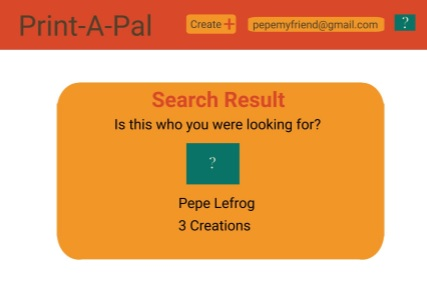
\includegraphics[width=\textwidth/2]{searchresults.jpg}
\end{center}
\paragraph{figure 1. Image of the search result page}
\paragraph{}
When first accessing the website, users are directed to the landing page.  From here, they can choose to sign in or register their accounts.  The blue avatar icon at the top right of the screen can also be clicked to bring you to the log in page, and the search bar can be used at any time to search for other accounts using the email address associated with their account.   When logged in, users are directed to their profile page, where they can edit their profile or change settings.  Users can additionally browse their past creations, or click the Create + button to start a new creation residing at the top of the menu once logged in.\\
 
\noindent In the browsing page, you can view any of your past creations to start working on them again.  Searching for users by email address brings you to the result page where a single user is displayed with their avatar, name and number of creations.  You can then click their profile to go to their profile page and browse their creations. \\
 
\noindent In the creation menu, users can use the available tools to design their creation, and can save their progress and exit or submit the creation to be printed in the order page. 
\section{Landing Page and Registration}

\begin{center}
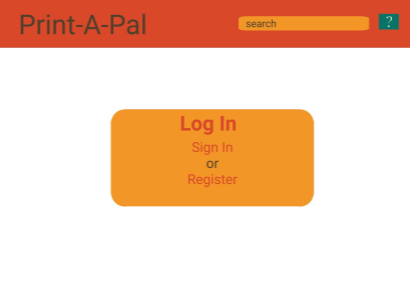
\includegraphics[width=\textwidth/2]{login.png}
\end{center}
\paragraph{figure 2. An image of the landing page/log in page}
The landing page, if not signed in, gives you the option to log in, register for an account, or search for other users by entering their email in the search menu. \\
 
\noindent In the registration page, users can register for their account with Print-A-Pal, by entering their email, desired password, name, and age (optional).  
\section{Profile Page}
\begin{center}
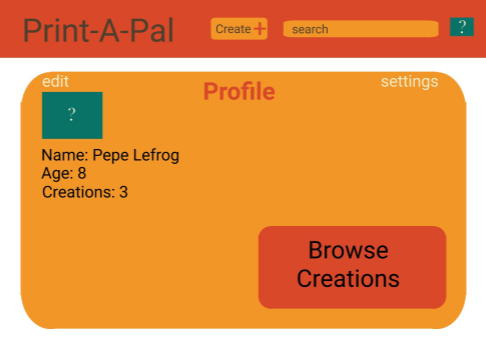
\includegraphics[width=\textwidth/2]{profile.png}
\end{center}
\paragraph{figure 3. An image of the profile page}
In the profile page, users are able to edit their profile, change their account settings, or click the Browse Creations button to browse the profile’s creations.  The name, age, and avatar are allowed to be changed in the edit profile section.  The application’s notifications, theme, and payment options are changeable from the account settings menu. 
 
\section{Browse Creations}
\begin{center}
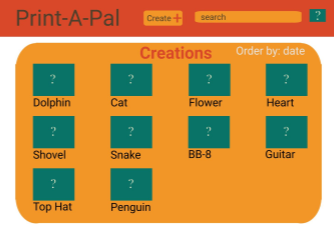
\includegraphics[width=\textwidth/2]{creations.png}
\end{center}
\paragraph{figure 4. An image of the browse creations page}
\paragraph{} In the browse creations page, users can choose in which order to cycle through their past creations, giving them the option to view or edit any of their work.  When browsing another user’s creations, users are only allowed to view the rendering in different angles and not able to change anything
\section{Order Page}
\begin{center}
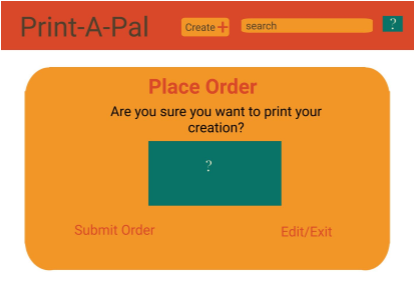
\includegraphics[width=\textwidth/2]{order.png}
\end{center}
\paragraph{figure 4. An image of the order page}
\paragraph{}In the order page, users are asked to confirm their choice of sending their work to be 3D printed, or go back to the creation page to edit their work further.  Choosing to submit order takes users to the payment and delivery section which enables them to place the order for their creation to be 3D printed. 
\section{Creation page}
In the creation page, users are given a variety of tools to work with to adjust and change the design of their creation.  There are two main views within the creation page: the front view and side view.  The front view is a 2D representation of the work space and where users do the majority of designing for their creation, drawing shapes onto the 2D plane.  In the side view, users are given a 3D side angle of their drawing, where they can adjust the thickness and roundness of the edges of the shapes they have created in the 2D front view.  The camera angle is adjustable to show different views of the image, unlike the 2D drawing view where users can only draw onto the 2D plane

\chapter{Module Decomposition}
\section{2D Drawing Module}
Set of drawing operations for 2D shapes
\subsection{createCircle(radius)}
Draws a circle of specified radius
\subsection{createRectangle(startX, startY, endX, endY)}
Draws a rectangle with the specified vertices.
\subsection{createLine(startX,startY,endX,endY)}
Draws a line with specified vertices.
\subsection{pencil(startX, startY, enable\_drag)}
Draws on canvas with pencil object.
\subsection{getCurrentMouseCoords(mouseX,mouseY)}
Get current mouse position.

\section{Math Library for 3D Objects and Planes}
Set of operations and objects for calculating 3D object primitives:
\subsection{Objects}
\subsubsection{Vector(x,y,z)}
Defines 3D vector object.
\subsubsection{Coord(x,y,z)}
Defines 3D coordinate object.
\subsubsection{Plane(x,y,z,d)}
Defines 3D plane object.
\subsection{Operations}
\subsubsection{normalVector(vec1, vec2)}
Calculates the normal vector given two vectors.
\subsubsection{vecMagnitude(vec)}
Calculates the magnitude of a vector.
\subsubsection{normalizeVec(normalizeVector)}
Returns normal form of vector.
\subsubsection{planeEq(coord1,cood2,coord3)}
Given 3 coordinates return the equation of a plane.

\section{3D Rendering Module for Planes and Objects}
Set of operations and objects drawing 3D primitives, meshes and objects.
\subsection{Objects}
\subsubsection{Mesh(length,drawfunc)}
Creates a mesh by initializing its array to the specified length and draws the mesh according to previously defined draw function.
\subsection{Operations}
\subsubsection{drawMesh(meshObject)}
Iterates over the mesh object daa structure and draws it.
\subsubsection{createsMesh(typeofMesh)}
Creates and returns a mesh object that can later be used with drawMesh().
\subsubsection{drawTri(coord1, coord2, coord3)}
Used to draw triangles for mesh objects.

\section{Custom 2D to 3D Projection Module}
\subsection{Objects}
\subsubsection{ViewMatrix and ProjectionMatrix}
These objects are used to calculate the projection.
\subsection{Operations}
\subsubsection{get2DPoint(coord1, ViewMatrix, ProjectionMatrix, length, width)}
Returns the 2D screen point of 3D scene world.
\subsubsection{get3DPoint(coord1, ViewMatrix, ProjectionMatrix, length, width)}
Returns the 3D world coordinate of a 2D projection point.

\section{Module for 3D mesh object to STL file}
Set of operations and objects that are used to convert a mesh object to an STL file format for 3D printing purposes.
\subsection{Objects}
\subsubsection{parseMesh(meshObject)}
Iterates through mesh object list for series of triangles and their respective face normal and returns STL file for the specified mesh object.

\section{User Management Module}
Set of operations and objects that associate a user object with their creations.  The objects in this section are also representative of schema definition.
\subsection{Objects}
\subsubsection{User(id, name, username, password)}
\subsubsection{Object3D(id, object\_type, project\_id, file\_id)}
\subsubsection{File(id, file\_url)}
\subsubsection{Project(id, user\_id)}
\subsection{Operations}
\subsubsection{createNewUSer(name,username,email,password,confirm\_pass)}
Creates a new user and saves it to database.
\subsubsection{deleteUser(id)}
Deletes the user from the database.
\subsubsection{editUser(id, options = \{\}}
Grabs the user by the id and the options hash can be used to edit the individual attributes that make up the user object and save it to database
\subsubsection{returnUser(id)}
Grabs the user by the ID.
\subsubsection{createNewFile()}
Creates a new File and saves the file\_url to the database.
\subsubsection{editFile(id, options = \{\}}
Grabs the file by the ID and the options hash can be used to edit the individual attributes that make up the user object and save it to database.
\subsubsection{deleteFile(id)}
Deletes file by ID from database.
\subsubsection{returnFile(id)}
Returns the file from the database according to its ID.


\chapter{Technology Stack Break Down}
\section{Front End}
We will be using the standard html/css/javascript stack with additional libraries to fully support the product’s functionality. We will use jquery library for basic javascript. We will also use three.js which is a javascript library for WebGL. For styling purposes will use bootstrap for consistent styling throughout the web application 
\section{Back End}
We will use ruby on rails framework since it has many operations within the framework already setup for starting up a web application. The framework will run off an nginx server. We will also use SQL database for information storage and retrieval and also C programming language for creating additional wrapper functions for the ruby on rails framework to support conversion from a 3D mesh object to a standard STL file.
\section{Additional APIs}
Wolfram Alpha library may be used for functions that are computationally intensive. Also we will use Amazon Web Services S3 module for storing files. The file URL will stored in the database. We will also use Heroku for hosting as it is already configured for Ruby on Rails Applications. 

\chapter{ER Diagram}
\begin{center}
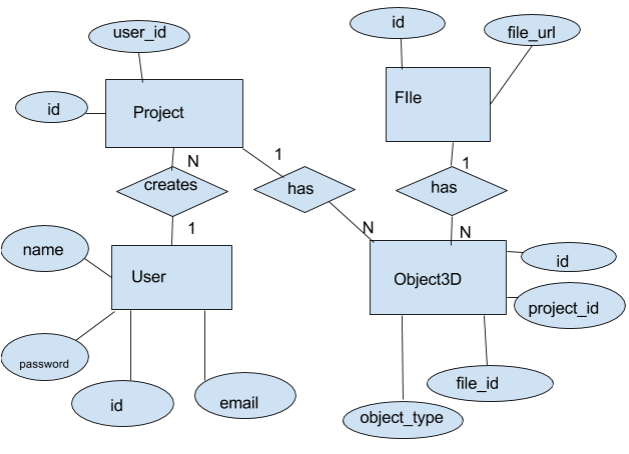
\includegraphics[width=\textwidth/2]{ER.png}
\end{center}
\paragraph{figure 3. An entity-relationship diagram of Print-A-Pal}
\end{document}












